\newpage
\chapter{Using Terminology to Improve Machine Translation}
\label{chap:terminmt}

Phrase-based Statistical Machine Translation (SMT) obtains the best translation by maximizing the conditional probability of the source sentence given the foreign sentence, $p(e|f)$. Using Bayesian deductions, we require the conditional probability of the foreign sentence given the source sentence and the a priori probability of the translation, $p_{LM}(e)$ (Brown, 1993); mathematically

\begin{equation}
arg\max _{  }{ p(e|f)=arg\max _{  }{ p(f|e)\cdot { p }_{ LM }(e) }  } 
\end{equation}


State-of-art SMT systems rely on (i) large bilingual corpora to train the translation model $p(f|e)$ and (ii) monolingual corpora to build the language model, $p_{LM}(e)$ (See Chapter 2, Section 2.2).

There are two primary approaches to the use of bilingual dictionary resources in statistical machine translation: (i) the \textbf{\textit{passive}} approach of appending the parallel training data with a bilingual dictionary and prior to traiing the SMT (ii) the \textbf{\textit{pervasive}} approach of enforcing translation as per the dictionary entries when decoding. 

Previous studies have shown that both approaches of providing external lexical knowledge to statistical machine translation show the potential of improving translation quality (See Chapter 2, Section 2.4.7). In this chapter, empirically investigate the effects of both approaches on the same dataset and provide further insights on how lexical information can be reinforced in statistical machine translation.

The \textbf{\textit{passive}} approach to improve the SMT model is to extend the parallel data with a bilingual dictionary prior to training the model. The primary motivation is to use additional lexical information for domain adaptation to overcome the this issue out-of-vocabulary words during decoding (Koehn and Schroeder, 2007; Meng et al. 2014; Wu et al. 2008). Alternatively, adding in-domain lexicon to parallel data has also shown to carry the potential to improve SMT. The intuition is that by adding extra counts of bilingual lexical entries, the word alignment accuracy improves, resulting in a better translation model (Skadins et al. 2013; Tan and Pal, 2014; Tan and Bond, 2014).

The \textit{\textbf{pervasive}} approach to use a bilingual dictionary is to hijack the decoding process and force word/phrase translations as per the dictionary entries. Previous research used this approach to explore various improvements in industrial and academic translation experiments to enhance specifically term translation consistency.

\section{Passive and Pervasive Lexical Injection}

We view both the passive and the pervasive use of a dictionary in statistical machine translation as a type of lexically constrained statistical MT where in the passive use, the dictionary acts a a supplementary set of bi-lexical rules affecting word and phrase alignments and the resulting translation model and in the pervasive use, the dictionary constraints the decoding search space enforcing translations as per the dictionary entries. 

To examine the \textbf{\textit{passive}} use of a dictionary, we explore the effects of adding the lexicon \textit{n} number of times to the training data until the performance of the machine translation degrades. For the \textbf{\textit{pervasive}} use of a dictionary, we assign a uniform translation probability to possible translations of the source phrase as determined by the dictionary. For instance, in a dictionary, the English term ``\textit{abnormal hemoglobin}” could be translated to 
\begin{CJK*}{UTF8}{min}異常 ヘモグロビン\end{CJK*} or 
\begin{CJK*}{UTF8}{min}異常血色素\end{CJK*}, 
we assign the translation probability of 0.5 to both Japanese translations uniformly, i.e. p(\begin{CJK*}{UTF8}{min}異常 ヘモグロビン\end{CJK*} | abnormal hemoglobin) = p(\begin{CJK*}{UTF8}{min}異常血色素\end{CJK*} | abnormal hemoglobin) = 0.5. If there is only one translation for a term in the dictionary, we force a translation from the dictionary by assigning the translation probability 1.0 to the translation.

One issue with the pervasive use of dictionary translations is the problem of compound phrases in the test sentence that are made up of component phrases in the dictionary. For instance, when decoding the sentence, ``\textit{Here was developed a phase shift \underline{magnetic sensor system} composed of two sets of coils , amplifiers , and phase shifts for sensing and output .}", we fetch the following entries from the dictionary to translate the underlined multiword term:

\begin{itemize}[noitemsep]
\item  magnetic = \begin{CJK*}{UTF8}{min}磁気\end{CJK*}
\item sensor = \begin{CJK*}{UTF8}{min}センサ, センサー, 感知器, 感知部, 感応素子, 検出変換器, 変換素子, 受感部, 感覚器, センサー\end{CJK*}
\item system = \begin{CJK*}{UTF8}{min}組織体制, 制度, 子系, 系列, シス
テム, 体系, 方式, 系統, 秩序, 体制, 組織,
一方式\end{CJK*}
\item  magnetic sensor = \begin{CJK*}{UTF8}{min}磁気センサ\end{CJK*}
\item  sensor system = \begin{CJK*}{UTF8}{min}センサシステム, センサ系, センサーシステム\end{CJK*}
\end{itemize}

In such a situation, where the dictionary does not provide a translation for the complete multi-word string, we set the preference for the dictionary entry with the longest character length in the direction from left to right and select “magnetic sensor” + “system” entries for forced translation. Finally, we investigate the effects of using the bilingual dictionary both passively and pervasively by appending the dictionary before training and hijacking the decoding by forcing translations using the same dictionary.

\subsection{Adding Single Word vs Multi-Word Dictionary Entries to SMT}

Since the phrase-based machine translation model capitalizes on the alignment `consistency’ which essentially requires asymmetric alignment points to extract phrases, it remains unclear whether mono-lexical entries affect the final machine translation quality and how they affect the probability mass during the phrase extraction process. We examine the effects of adding only single word entries vs only adding multi-word entries from the dictionary to the SMT training data to compare the difference between using the full bilingual dictionary vs the mono-lexical or multi-word versions.

% Pikachu, Domosaur, and other Monolexical Languages: http://sigbovik.org/2014/proceedings.pdf

\subsection{Adding a Manually Crafted Dictionary vs an Automatically Extracted Terminology to SMT}

From the literature,\footnote{See Chapter 2 Section 2.3} the popular approach to adding lexical information to statistical machine translation is to passively add automatically extracted a bilingual dictionary / terminology resources to SMT training data. The intrinsic quality of the automatically extracted bilingual dictionary is often disregarded since the ultimate interest is to achieve a BLEU score increment. In the Chapter 3, we experimentally show that both the intrinsic and extrinsic evaluation of the automatically extracted terminology resource using the $PMI_{LM}$ term extraction statistics. 

In the following result section, we would like to explore the difference between using an automatically extracted terminology and a manually crafted dictionary. We use the global $PMI_{LM}$ extraction method described in Chapter 3 to extract the top 100,000 terms to be used as our automatically extracted terminology.

\subsection{Experimental Setup}

We experimented with the passive and pervasive uses of dictionary resources in SMT using the Japanese-English dataset provided in the Workshop for Asian Translation (Toshiaki et al. 2014). We used the Asian Scientific Paper Excerpt Corpus (ASPEC) as the training corpus used in the experiments. The ASPEC corpus consists of 3 million parallel sentences extracted from Japanese-English scientific abstracts from Japan’s Largest Electronic Journal Platform for Academic Societies (J-STAGE). In our experiments we follow the setup of the WAT shared task with 18,00 development and test sentences each from the ASPEC corpus. 

We use the manually crafted Japanese-English (JA-EN) translation dictionaries (JICST, 2004) from the Japan Science and Technology Corporation. It contains 800,000 entries for technical terms manually extracted from scientific and technological documents. 

Similarly, we use the bilingual $PMI_{LM}$ term extractor (from Chapter 3) to extract the top 800,000 terms from the training corpus. We seek to compare the efficacy of the manually crafted dictionary versus the automatically extracted one when using incorporating lexical information in the training data passively and pervasively. 

From Chapter 4.5, in Table 4.5, we note that adding the top 10,000 terms extracted using the $PM_{LM}$ reports statistically significant improvements from the baseline. While the experiment in Chapter 4.5 was concerned about how many unique terms to add to the training data for SMT, the experiments in this chapter using the automatically extracted terms focus on the number of times the extracted terminology is added to the training data for SMT. 

For parity in comparing automatically extracted and manually crafted dictionary resources, we compute the $PMI_{LM}$ values for all entries and extracted the 10,000 terms from the manually crafted dictionary. 

The parallel data, the manually crafted bilingual dictionary and automatically extracted terminology are all tokenized with the MeCab segmenter (Kudo et al. 2004). We use the phrased-based machine translation configuration as described in Chapter 2, Section 2.4.4. 

For the \textit{passive} use of the dictionary, we simply appended the dictionary resources to the training data before the alignment and training process. For the \textit{pervasive} use of the dictionary, we used the {\tt xml-input} function in the Moses toolkit to force lexical knowledge in the decoding process.

Different from the normal use of a dictionary for the purpose of domain adaptation where normally, a domain-specific lexicon is appended to a translation model trained on generic texts, we are investigating the use of an in-domain dictionary in statistical machine translation.

More specifically, we seek to understand how much improvement can be made by skewing the lexical information towards the passive and pervasive use of the dictionary without additional domain knowledge i.e the dictionary comes from the same domain as the training corpus.

\subsection{Results (Passive vs Pervasive)}

\begin{table}[H]
\centering
    \begin{tabular}{l|ll}
    ~           & \textbf{-Pervasive} &\textbf{ +Pervasive }\\ \hline
    \textbf{Baseline}    & 16.75      & 16.87      \\ \hline
    \textbf{Passive x 1 }& 16.83      &  17.30$^{**}$   \\
    \textbf{Passive x 2} & \textbf{17.31$^{**}$}    & 16.87      \\
    \textbf{Passive x 3 }&  17.26$^{*}$    & 17.06      \\
    \textbf{Passive x 4 }& 17.14$^{*}$     &  \textbf{17.38$^{**}$}   \\
    \textbf{Passive x 5 }& 16.82      &  17.29$^{**}$   \\
    \end{tabular}
\caption{BLEU Scores for Passive and Pervasive Use of the Dictionary in SMT (Japanese to English)}
\label{table:hytrajaen}
\end{table}

Table 4.1 presents the BLEU scores of the Japanese to English (JA-EN) translation outputs from the phrase-based SMT system on the WAT test set. The \textbf{-Pervasive} column indicates the number of times a dictionary is appended to the parallel training data (Baseline = 0 times, Passive x$n$ = $n$ time). The \textbf{+Passive} column presents the results from both the passive and pervasive use of dictionary translations, with the exception to the top-right cell which shows the baseline result of the pervasive dictionary usage without appending any dictionary to the training data.

By repeatedly appending the dictionary to the parallel data, the BLEU scores significantly\footnote{*: p-value<0.1, **: p-value<0.001} improves over the baseline from 16.75 to 17.31. Although the system’s performance degrades when adding the dictionary passively thrice, the score remains significantly better than baseline. The pervasive use of the dictionary marginally improves the baseline without the passive use of the dictionary. The best performance is achieved when the dictionary is passively added four times with the pervasive use of the dictionary during decoding.

The small fluctuations in improvement from coupling the passive and pervasive use of an in-domain dictionary give no indication of how both approaches should be used in tandem. However, using either or both the approaches improves the translation quality over the baseline system.

\begin{table}[H]
\centering
    \begin{tabular}{l|ll}
    ~           & \textbf{-Pervasive} &\textbf{ +Pervasive }\\ \hline
    \textbf{Baseline}    & 23.91      & 23.14$^{**}$      \\ \hline
    \textbf{Passive x 1 }& 24.12$^{*}$     &  23.13$^{**}$   \\
    \textbf{Passive x 2} & 23.79    & 22.86$^{**}$      \\
    \textbf{Passive x 3 }&  \textbf{24.14$^{*}$}   & \textbf{23.29$^{**}$}      \\
    \textbf{Passive x 4 }& 24.13$^{*}$     &  23.16$^{**}$   \\
    \textbf{Passive x 5 }& 23.67      &  22.71$^{**}$   \\
    \end{tabular}
\caption{BLEU Scores for Passive and Pervasive Use of the Dictionary in SMT (English to Japanese)}
\label{table:hytraenja}
\end{table}

Table 4.2 presents the BLEU scores of the English to Japanese (EN-JA) translation outputs from the phrase-based SMT system on the WAT test set. The passive use of dictionary outperforms the baseline. Different from the JA-EN translation the pervasive use of dictionary consistently performs worse than the baseline. Upon random manual checking of the MT output, there are many instances where the technical/scientific term in the dictionary is translated correctly with only the passive use of the dictionary. However, it is unclear whether the overall quality of the translations have degraded from the pervasive use of the dictionary given the slight, though significant,\footnote{*: p-value<0.1, **: p-value<0.001} decrease in BLEU scores.

%\vspace{-5mm}
\begin{figure}[!htb]
\centering
	\hspace{-2em}%
	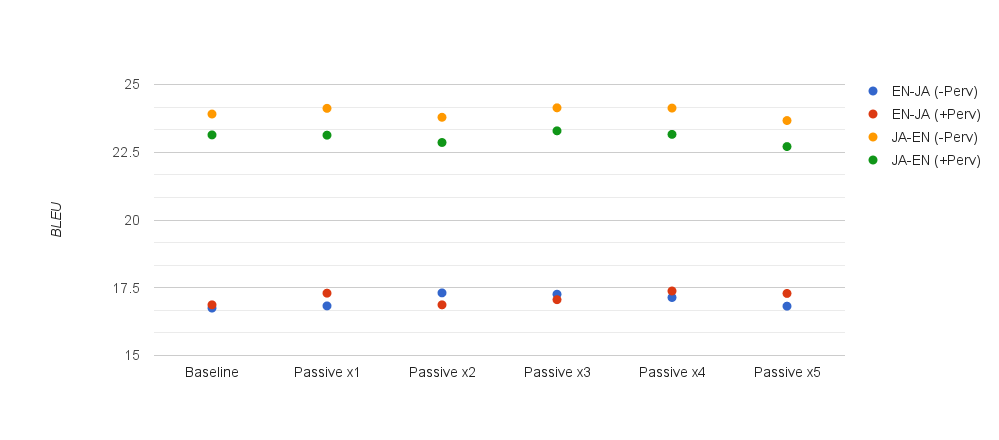
\includegraphics[width=15cm]{hytra.png} \\[-1em]
	\caption{Overview of the Passive and Pervasive Use of Dictionary in the WAT Experiments}
	\label{fig-hytra}
\end{figure}

Figure 4.1 summarizes the results of our experiments on passive and pervasive use of manually created JIST dictionary with the ASPEC corpus evaluated with the WAT evaluation test set. Empirically, both passive and pervasive use of an in-domain dictionary to extend statistical machine translation models with lexical knowledge modestly improve translation quality. Interestingly, the fact that adding the in-domain dictionary information multiple times to the training data improves MT suggests that there may be a critical probability mass by increasing the frequency of in-domain terms which can impact the word and phrasal alignments in a corpus. This may provide insight on optimizing the weights of the salient in-domain phrases in the phrase table.

Although the pervasive use of dictionary information provides minimal or no improvements to the BLEU scores in our experiments, it remains relevant in industrial machine translation where terminological standardization is crucial in ensuring consistent translations of technical manuals or legal texts where incorrect use of terminology may have legal consequences (Porsiel, 2011).

\subsection{Results (Mono-lexeme vs Multi-Word Expressions)}

In a further experiment motivated in Section 4.1.1, we seek to examine the difference between adding mono-lexical entries and multi-word expressions. Table 4.3 presents the results of the experiments on passively adding subsets of the dictionary instead of the full JIST dictionary. The first column (\textbf{Mono-Lexeme}) of Table 4.3 indicates the number of times the mono-lexical entries from the dictionary is appended to the parallel training data (Baseline = 0 times, Passive x1 = 1 time, etc.). The \textbf{Multi-words} column presents the results from adding the multi-word entries from the dictionary to the data before the statistical machine translation training process. The last column of results (\textbf{Full}) in Table 4.3 is the same as the first results column in Table 4.1.

\begin{table}[H]
\centering
    \begin{tabular}{l|lll}
         ~               & \textbf{Mono-Lexeme} & \textbf{Multi-Words} & \textbf{Full} \\ \hline
\textbf{Baseline}        & 16.75      & 16.75      & 16.75  \\ \hline
    \textbf{Passive x1}  & 16.82$^{*}$       & 16.99$^{**}$   & 16.83     \\
    \textbf{Passive x2}  & 16.81$^{*}$       & 16.59     & \textbf{17.31$^{**}$}  \\
    \textbf{Passive x3}  & \textbf{17.01}    & \textbf{17.03}     &  17.26$^{*}$  \\
    \textbf{Passive x4}  & 16.67       & 17.01    & 17.14$^{*}$   \\
    \textbf{Passive x5}  & 16.54       & 16.96    & 16.82   \\
    \end{tabular}
\caption{BLEU Scores in adding Mono-lexeme vs MWE Dictionary to SMT (English to Japanese)}
\label{table:mumtttaenja}
\end{table}

Table 4.3 shows that it is possible to achieve slight statistically significant though marginal improvements from baseline (16.75) by adding the single word once or twice. Adding multi-word entries to the training data also makes statistically significant and marginal improves only when added once. Extending the training data with the full manually crafted dictionary makes the lexical addition more robust and the SMT system makes statistically significant improvements when the dictionary is added 2 to 4 times; the best score (17.31) is achieved when the full dictionary is added twice.

Here we identify a gap in the current strain of research focusing on passively adding only multi-word expressions to SMT training process. Intuitively, we may conjecture that that having mono-lexical entries (e.g. \textit{magnetic = \begin{CJK*}{UTF8}{min}磁気\end{CJK*} sensor = \begin{CJK*}{UTF8}{min}センサ\end{CJK*}; system = \begin{CJK*}{UTF8}{min}シス\end{CJK*}}) that make up the partial multi-word expressions (\textit{magnetic sensor = \begin{CJK*}{UTF8}{min}磁気 センサ\end{CJK*};  sensor system = \begin{CJK*}{UTF8}{min}センサ システム\end{CJK*}}) help in word/phrase alignment process, improving the overall translation quality. But this intuition seems to only hold when translating from English to Japanese. 

\begin{table}[H]
\centering
    \begin{tabular}{l|lll}
         ~               & \textbf{Single Word} & \textbf{Multi-Words} & \textbf{Full} \\ \hline
\textbf{Baseline}        & 23.91      &  23.91      & 23.91  \\ \hline
    \textbf{Passive x1}  & \textbf{23.93}      & 23.96   & 24.12$^{*}$     \\
    \textbf{Passive x2}  & 23.87      & 24.01     & 23.79  \\
    \textbf{Passive x3}  & 23.54   & \textbf{24.14$^{**}$ }    &  \textbf{24.14$^{*}$}  \\
    \textbf{Passive x4}  & 22.91$^{**-}$       & 23.92    & 24.13$^{*}$   \\
    \textbf{Passive x5}  & 23.35       & 23.87$^{**-}$    & 23.67   \\
    \end{tabular}
\caption{BLEU Scores in adding Single Words vs Multi-Words Dictionary to SMT (Japanese to English)}
\label{table:mumtttjaen}
\end{table}

\begin{figure}[H]
\centering
	\hspace{-2em}%
	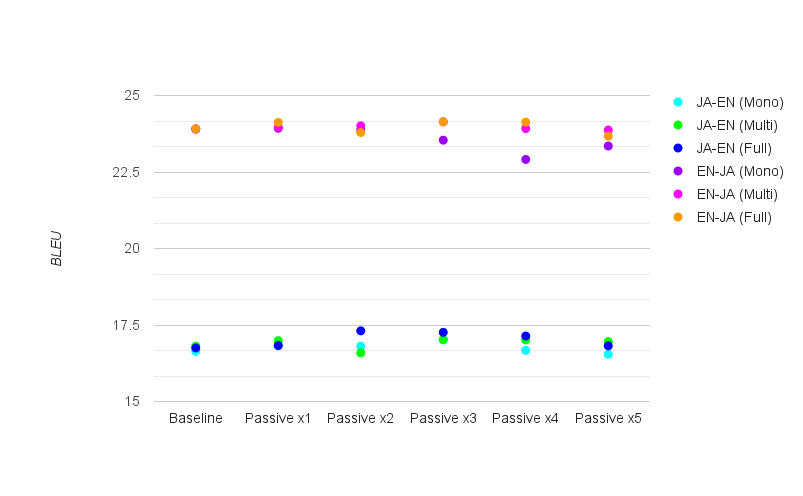
\includegraphics[width=15cm]{mumttt.png} \\[-1em]
	\caption{Overview of the Mono-Lexeme and Mult-Word Expression subset of the Dictionary in the WAT Experiments}
	\label{fig-mumttt}
\end{figure}
\vspace{-5mm}

Table 4.4 compares the results of adding the mono-lexical vs multi-word entries from the dictionary in the attempt to improve BLEU scores\footnote{*: p-value<0.1, **: p-value<0.001}\footnote{*-: p-value<0.1 with negative BLEU from baseline, **-: p-value<0.001 with negative BLEU from baseline}. Interestingly, when translating from Japanese to English, the mono-lexical entries marginally reported lower BLEU scores as compared to the MWEs. And by adding only the multi-word entries, the SMT system achieves similar results to using the full dictionary.

Figure 4.2 summarizes our experiments comparing the addition of mono-lexical and multi-word entries to the statistical machine translation training process. Empirically, we have shown that the usage of the full dictionary might not be necessary depending on the directionality of translation.

\subsection{Results (Manual vs Automatic)}

\begin{table}[H]
\centering
    \begin{tabular}{l|ll|ll}
               & \textbf{JICST} & \textbf{PMI\_LM} & \textbf{JICST} & \textbf{PMI\_LM }  \\ 
                & \textbf{(800k)} & \textbf{(800k)} & \textbf{(10k)} & \textbf{(10k)}  \\ \hline
\textbf{Baseline}  & 16.75 & 16.75 & 16.75 & 16.75 \\ \hline           
                
    \textbf{Passive x1} & 16.83        & 15.34$^{*-}$          & 16.16       & \textbf{16.81}         \\
    \textbf{Passive x2} & \textbf{17.31$^{**}$ }       & 14.82$^{**-}$          & 16.23       & 16.73   \\
    \textbf{Passive x3} & 17.26$^{*}$        & \textbf{15.90$^{*-}$}          & \textbf{16.28}       & 15.68$^{**-}$    \\
   \textbf{Passive x4} & 17.14$^{*}$        & 14.32$^{**-}$          & 15.76$^{*-}$       & 15.54$^{**-}$    \\
    \textbf{Passive x5} & 16.82        & 13.87$^{**-}$          & 15.12$^{*-}$       & 14.91$^{**-}$       
    \end{tabular}
    \caption{BLEU Scores in passively adding a Manually Crafted Dictionary vs an Automatically Extracted Terminology to SMT (English to Japanese)}
\label{table:watlmpmienja}
\end{table}


Table 4.5 shows the result of passively adding a manually crafted dictionary (JICST) against an automatically extracted terminology using $PMI_{LM}$ when translating from English to Japanese. For the comparison that follows, we will keep in mind that our baseline system without adding additional lexical knowledge scores 16.75 BLEU (from Table 4.1) and the significance results\footnote{*: p-value<0.1, **: p-value<0.001}\footnote{*-: p-value<0.1 with negative BLEU from baseline, **-: p-value<0.001 with negative BLEU from baseline} presented on Table 4.5 are with respect to this baseline system.

The \textbf{JICST (800K)} and \textbf{$PMI_{LM}$ (800K)} columns in Table 4.5 shows the results we presented on Table 4.1 when passively adding the full hand-crafted JICST dictionary to the training data and the second column shows the BLEU scores achieved by the same SMT configurations except that we passively add the top 800,000 terms automatically extracted terminology using $PMI_{LM}$. Table 4.5 that all results from passively adding the automatically extracted terms performed significantly worse than the baseline system that scored 16.75 BLEU.

The \textbf{JICST (10K)} and \textbf{$PMI_{LM}$ (10K)}  columns in Table 4.5 present another setting where we added the top 10,000 entries from the manually crafted dictionary ranked by their $PMI_{LM}$ values and an automatically extracted terminology with $PMI_{LM}$ with 10,000 terms. We achieved the best results (16.81 BLEU) when passively adding the automatically extracted terms just once. Although the absolute BLEU score is marginally higher than our baseline (16.75 BLEU), the increment is not significant. Likewise using the smaller subset of the manually crafted dictionary underperforms as compared to using the full dictionary. 

Statistical significance measures the difference of the output of a system from the output of the baseline system. While the negative results of adding automatically extracted terminology are statistically significant, the BLEU score fluctuations are marginal. The overall results did not give a clear signal as to whether adding an automatically extracted dictionary is beneficial or detrimental to the SMT system. 

\begin{figure}[!htb]
\centering
	\hspace{-2em}%
	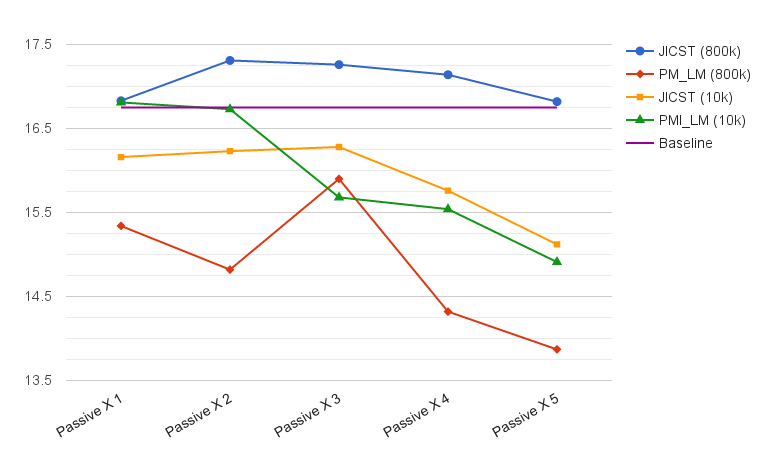
\includegraphics[width=15cm]{dict-term.png} \\[-1em]
	\caption{Passively Adding a Manually Crafted Dictionary vs an Automatically Extracted Terminology (English-Japanese)}
	\label{fig-manvauto}
\end{figure}

Figure 4.3 provides a visual description for Table 4.5. From Figure 4.3, it is more evident that adding the additional lexical information once is optimal when using an automatically extracted terminology (referring to the first green-triangle data point). BLEU scores quickly degrades once we add the 10k terms  more than two times. 

Unsurprisingly, when we filter out the top 10k entries from the manually crafted dictionary, it underperformed as compared to using the full dictionary. However, we see a marginally upwards trend in BLEU scores as we add the dictionary once and twice. This suggests the \textit{`effective multiplier'} idea that (Brown et al., 1993a) proposed\footnote{See Chapter 2, Section 2.3.1}.

The narrative changes when we increase the size of the terminology to 800k, passively adding the automatically extracted terminology thrice performs the best but other than this small anomaly, adding the  terminology follows a linear downwards trend\footnote{Possibly, the fluke in BLEU when passively adding the terminology thrice is caused by the non-deterministic MERT tuning process that found better optimum weights.}. From previous experiments varying the size of the terminology (Chapter 3, Section 3.5), we see that using the top 10,000 terms performed better than 12,000 terms for both English-Japanese and Japanese-English translation\footnote{They are trained and evaluated on the same ASPEC corpus and WAT evaluation dataset}. Thus increasing the size of terminology to 800,000 would just be adding more noise to the system. Interestingly, we see that the phrase-based machine translation is rather robust to the noisy $~$70,000 bilingual terms that we've added and report only slight decrease in BLEU scores. 

\begin{table}[H]
\centering
    \begin{tabular}{l|ll|ll}
               & \textbf{JICST} & \textbf{PMI\_LM} & \textbf{JICST} & \textbf{PMI\_LM} \\ 
               & \textbf{(800k)} & \textbf{(800k)} & \textbf{(10k)} & \textbf{(10k)} \\ \hline
 \textbf{Baseline}  & 23.91 &23.91  & 23.91 & 23.91 \\ \hline
    \textbf{Passive x1} & 24.12$^{*}$        & 23.26$^{*-}$          & \textbf{23.85}       & \textbf{23.78}        \\
   \textbf{Passive x2} & 23.79        & \textbf{23.45}          & 23.72       & 23.76      \\
    \textbf{Passive x3} & \textbf{24.14$^{*}$ }       & 22.81$^{*-}$          & 22.84$^{*-}$       & 22.93$^{*-}$       \\
    \textbf{Passive x4} & 24.13$^{*}$        & 22.35$^{*-}$          & 23.04$^{*-}$       & 23.01$^{*-}$         \\
    \textbf{Passive x5} & 23.67        & 21.93$^{*-}$          & 22.91$^{*-}$       & 23.00$^{*-}$   
    \end{tabular}
    \caption{BLEU Scores in adding Manually Crafted Dictionary vs Automatically Extracted Terminology to SMT (Japanese to English)}
\label{table:watlmpmijaen}
\end{table}

Table 4.6 shows the result of passively adding a manually crafted dictionary (JICST) against an automatically extracted terminology using $PMI_{LM}$ when translating from Japanese to English. For the comparison that follows, we will bear in mind that our baseline system without adding additional lexical knowledge scores 23.91 BLEU (from Table 4.2) and the presented on Table 4.5 are respectively to this baseline system.

\vspace{-5mm}
\begin{figure}[!htb]
\centering
	\hspace{-2em}%
	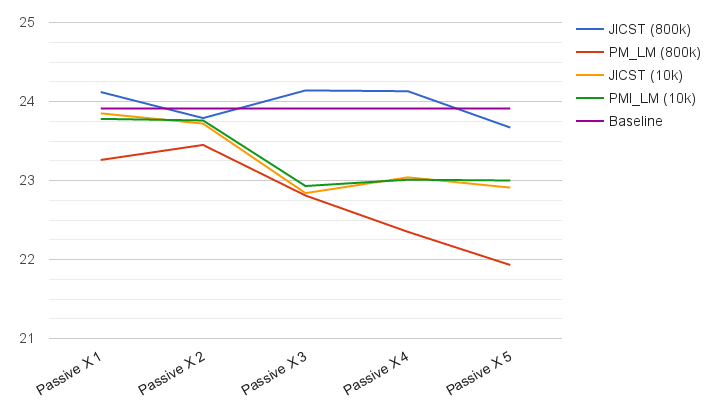
\includegraphics[width=15cm]{term-dict.png} \\[-1em]
	\caption{Passively Adding Manually Crafted Dictionary vs Automatically Extracted Terminology (Japanese-English)}
	\label{fig-manvauto}
\end{figure}

Figure 4.4 presents the results better graphically. similar to translating from English to Japanese, the best performance is achieved by passively adding manually crafted dictionary (BLEU 24.14), in this case adding it thrice. We see the same robustness of the SMT system given the noisy lexical information as the BLEU score drops marginally though the deterioration is statistically significant. 

In contrast to passively adding 800k automatically extracted terms  when translation from EN-JA, we see a slight increase in BLEU 23.26 -> 23.45  when the 800k terms were added twice. However, the same linearly degenerate behavior happens as we continue to passively increase the effective multiplier. 

As we reduce to the automatically extracted terminology size and the manually crafted dictionary size to 10k, we see that we achieved better results but still lower than the baseline (23.91 BLEU). But this does not come as a surprise since the best possible results from adding lexical information comes from adding the full JICST dictionary and it scantily improves upon the baseline system 23.91 -> 24.14.

\section{Summary}

In this chapter, we explore the multiple facade to integrate lexical information to phrase-based statistical machine translation  from (i) comparing passive and pervasive techniques, to understanding (ii) the synergy in using both mono-lexical and multi-word entries in passively adding lexicon to the SMT process and (iii) the difference in adding manually crafted versus automatically extracted lexicon to the SMT training data. 

In general, passively adding additional lexical information to statistical machine translation performs better than pervasively forcing the machine translation decoder to use the bilingual lexicon entries. To achieve optimal `effective multiplier' effect in passively addition lexicon to machine translation, we found that adding the lexicon more than once improves the performance; in our experiments, we found that adding 3-4 times yields the best result. Additionally, adding manually crafted dictionaries outperforms automatically extracted dictionaries. 



\iffalse
\section{Experiments on Workshop for Machine Translation (WMT) Dataset}
    \subsection{Using Named Entities and MWE for EN-HI Translations}
    \subsection{Using JRC Named Entities for EN-RU Translations}
\fi
    